%%%%%%%%%%%%%%%%%%%%%%%%%%%%%%%%%%%%%%%%%%%%%%%%%%%%%%%%%%%%%%%%
%
%  Template for creating scribe notes for cs229t. borrowed from Rob Schapire 
%
%  Fill in your name, lecture number, lecture date and body
%  of scribe notes as indicated below.
%
%%%%%%%%%%%%%%%%%%%%%%%%%%%%%%%%%%%%%%%%%%%%%%%%%%%%%%%%%%%%%%%%


\documentclass[11pt]{article}
\usepackage{mathtools,amssymb,amsthm}
\usepackage{enumerate}
%\usepackage[numbers]{natbib}
\usepackage{hyperref}
\usepackage{xcolor}
\hypersetup{
	colorlinks	= true,
	urlcolor	= orange,
	citecolor	= blue,
	linkcolor	= red
}
\usepackage{subfigure} 

\setlength{\topmargin}{0pt}
\setlength{\textheight}{9in}
\setlength{\headheight}{0pt}
\setlength{\headsep}{0pt}
\setlength{\oddsidemargin}{0.25in}
\setlength{\textwidth}{6in}

\newcommand{\draftnotice}{\vbox to 0.25in{\noindent
   \raisebox{0.6in}[0in][0in]{\makebox[\textwidth][r]{\it
    DRAFT --- a final version will be posted shortly}}}
   \vspace{-.25in}\vspace{-\baselineskip}
}

\pagestyle{plain}

\begin{document}

\thispagestyle{empty}

% \draftnotice

\begin{center}
\bf\large CS229T/STATS231: Statistical Learning Theory
\end{center}

\noindent
Lecturer: Tengyu Ma   %%% FILL IN LECTURER (if not RS)
\hfill
Lecture \#3               %%% FILL IN LECTURE NUMBER HERE
\\
Scribe: Mingda Qiao                 %%% FILL IN YOUR NAME HERE
\hfill
October 1, 2013           %%% FILL IN LECTURE DATE HERE

\noindent
\rule{\textwidth}{1pt}

\medskip

%%%%%%%%%%%%%%%%%%%%%%%%%%%%%%%%%%%%%%%%%%%%%%%%%%%%%%%%%%%%%%%%
%% BODY OF SCRIBE NOTES GOES HERE
%%%%%%%%%%%%%%%%%%%%%%%%%%%%%%%%%%%%%%%%%%%%%%%%%%%%%%%%%%%%%%%%

\newcommand{\A}{\mathcal{A}}
\newcommand{\argmin}{\operatorname*{argmin}}
\newcommand{\Ex}[2]{\mathbb{E}_{#1}\left[#2\right]}
\renewcommand{\H}{\mathcal{H}}
\newcommand{\poly}{\mathrm{poly}}
\newcommand{\pr}[2]{\Pr_{#1}\left[#2\right]}
\newcommand{\real}{\mathbb{R}}
\newcommand{\size}{\mathrm{size}}
\newcommand{\X}{\mathcal{X}}
\newcommand{\Y}{\mathcal{Y}}

\newtheorem{theorem}{Theorem}
\newtheorem{lemma}[theorem]{Lemma}
\newtheorem{definition}[theorem]{Definition}
\newtheorem{remark}[theorem]{Remark}

\section{Review and Overview}

In the first half of this course, the central question that we want to answer is: \emph{Why minimizing the training error often leads to a small testing error?} In the last lecture, we proved the asymptotics of the maximum likelihood estimator (MLE). In particular, as the number of training examples, denoted by $n$, tends to infinity,
	\[L(\hat\theta) - L(\theta^*) \approx \frac{p}{2n} + o\left(\frac{1}{n}\right).\]
Here $L$ is the expected loss. $\hat \theta$ is the minimizer of the training loss, while $\theta^*$ is the ground truth parameter. This result partially explains why the MLE, which has the smallest training loss, is also likely to achieve a small testing error when there are enough training examples.

One limitation of the above result is that it requires well-specifiedness, i.e., the data are distributed precisely according to a particular ground truth parameter $\theta^*$ in the parameter space. We would like to prove a more general result in the following form without assuming well-specifiedness.\footnote{In this case, $\theta^*$ needs to be redefined as the minimizer of the expected loss.}
	\[L(\hat\theta) - L(\theta^*) \le f(p, n), \forall p, n \ge 1.\]

Another limitation of this asymptotic result is that it ignores the dependence of higher order terms on other hyperparameters (in this case, the dimension $p$). Consider the following two functions, both of which are of order $\frac{p}{2n} + o\left(\frac{1}{n}\right)$:
	\[\frac{p}{2n} + \frac{1}{n^2} \quad \textrm{vs} \quad \frac{p}{2n} + \frac{p^{100}}{n^2}.\]
Arguably, the first one is a better upper bound since the second bound requires $n > p^{50}$ training examples to be below $1$.

From now on, we restrict our attention to the non-asymptotic regime, where $n$ is finite. In this lecture, we preview the form of results that we would like to prove in the following few lectures. Then we introduce the \emph{uniform convergence} framework, which we will instantiate in various settings to prove generalization bounds. We end this lecture by proving uniform convergence on finite hypothesis classes.

\section{Notations}
In the non-asymptotic setting, we only ignore the absolute constants (also known as universal constants). Specifically, whenever notation $O(X)$ appears in a statement, it means that there exists a universal constant $c$ such that the statement holds if we replace ``$O(X)$'' by $c\cdot X$. Similarly, we write $A \lesssim B$ as a shorthand for $A \le O(B)$.

In the following, we review a few central notations from previous lectures.
\begin{itemize}
	\item Hypothesis space: $\H$ is a family of hypotheses, i.e., prediction functions.
	\item Loss function: $\ell: (\X \times \Y) \times \H \to \real$. This is analogous to the notation $\ell((x, y), \theta)$ for loss functions in the last lecture, yet it accommodates the general case where we cannot naturally parametrize $\H$ by a continuum of parameters.
	\item Expected loss: $L(h) = \Ex{(x, y)\sim P}{\ell((x, y), h)}$, where $P$ is a data distribution over $\X \times \Y$. Moreover, we define $h^* \in \argmin_{h \in \H}L(h)$ as the minimizer of the expected loss.
	\item Training loss (also known as empirical risk): $\hat L(h) = \frac{1}{n}\sum_{i=1}^{n}\ell\left(\left(x^{(i)}, y^{(i)}\right), h\right)$, where
		$\left(x^{(1)}, y^{(1)}\right), \left(x^{(2)}, y^{(2)}\right), \ldots, \left(x^{(n)}, y^{(n)}\right)$
	are $n$ training examples drawn i.i.d. from $P$.
	\item Empirical risk minimizer (ERM): $\hat h \in \argmin_{h\in\H}\hat L(h)$.
\end{itemize}

\begin{remark}\label{rem:dependence}
	For a fixed data distribution $P$, there is no randomness in $h^*$, since $h^*$ is just the minimizer of a deterministic function $L(h)$. On the other hand, $\hat h$ is indeed a random variable, as the training loss function $\hat L$ is defined based on the training examples.

	The dependence between some of the above concepts is depicted in the following diagram:
	\begin{center}
		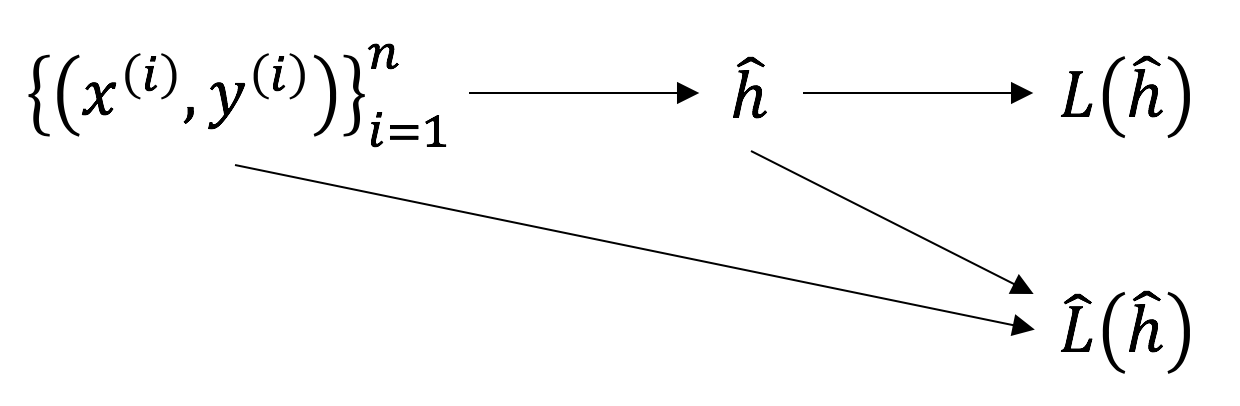
\includegraphics[scale=0.4]{1.png}
	\end{center}
\end{remark}

\section{Objective}
Our goal is to prove an upper bound on $L(\hat h) - L(h^*)$, the difference between the expected loss of the ERM $\hat h$ and that of the optimal hypothesis $h^*$. In particular, the results that we are going to prove in this and the following lectures are of the following form:
\begin{equation*}
	\pr{}{L(\hat h) - L(h^*) > \epsilon} \le \delta.
\end{equation*}
In words, with probability at least $1 - \delta$, it holds that $L(\hat h) - L(h^*) \le \epsilon$.\footnote{Here and in the following, the probability is always taken over the randomness in training examples unless otherwise specified.}

We can interpret $L(\hat h) - L(h^*) > \epsilon$ as a ``failure event'' since it means that the ERM $\hat h$ has an excess risk greater than parameter $\epsilon$, which is undesirable. Therefore, we would like the probability of this failure event to be as small as possible. Moreover, the smaller $\epsilon$ is, the stricter we are when evaluating the performance of $\hat h$. Thus, we would like parameters $\epsilon$ and $\delta$ to be as small as possible, given a fixed number of training examples.\footnote{As a general rule of thumb, we can make $\delta$ inverse polynomially small without using too many training examples, while the cost of minimizing $\epsilon$ is generally higher.}

Recall the definition of the ERM $\hat h$. We have
	\[\hat L(\hat h) = \min_{h \in \H}\hat L(h) \le \hat L(h^*).\]
In order to prove a high-probability bound of form
	\[L(\hat h) \le L(h^*) + \textrm{[extra term]},\]
it remains to argue that $\hat L(\hat h) \approx L(\hat h)$ and $\hat L(h^*) \approx L(h^*)$ (up to a small additive error) with high probability.

Proving $\hat L(h^*) \approx L(h^*)$ is relatively simple: 
	$\hat L(h^*) = \frac{1}{n}\sum_{i=1}^{n}\ell((x^{(i)}, y^{(i)}), h^*)$
is the average of $n$ i.i.d. random variables, each with expectation $L(h^*)$,
so we can prove a bound of the following form by applying standard concentration inequalities:
	\[\pr{}{\left|\hat L(h^*) - L(h^*)\right| \le \epsilon} \ge 1 - \delta.\]
In fact, this argument holds for \emph{any} fixed hypothesis $h \in \H$, as long as $h$ does not depend on the training examples.

The difficulty is in proving $\hat L(\hat h) \approx L(\hat h)$ since $\hat h$ is indeed a random variable that depends on the training examples (see Remark~\ref{rem:dependence}). Instead of a concentration bound for a single fixed hypothesis $h$, we need a stronger concentration property that holds for \emph{every} hypothesis in $\H$ simultaneously. This is where the notion of uniform convergence comes into play.

\section{Uniform Convergence}
Uniform convergence is a property of the hypothesis class $\H$ of the following form:
\begin{equation}
  \label{equation:uc}
  \pr{}{\forall h \in \H, \left|\hat L(h) - L(h)\right| \le \epsilon} \ge 1 - \delta.
\end{equation}
In words, it states that with probability at least $1 - \delta$ over the random draw of training data, the training loss is pointwise close to the expected loss, up to an additive error of at most $\epsilon$.

In general, if we parametrize the hypothesis space by $\real$, we would expect the picture of training loss and expected loss to be as in Figure~\ref{fig:1} if uniform convergence holds. It turns out that for particular learning tasks, the training loss exhibits a nicer landscape: it is not only pointwise close to the expected loss but also of the same shape, which is informally depicted in Figure~\ref{fig:2}. (See~\cite{ge2016matrix,mei2018landscape} for some of the recent work along this line of research.) Nevertheless, as only uniform convergence is concerned in this lecture, we do not distinguish these two different landscapes.

\begin{figure}[h]
	\centering
	\subfigure[]{
		\label{fig:1}
		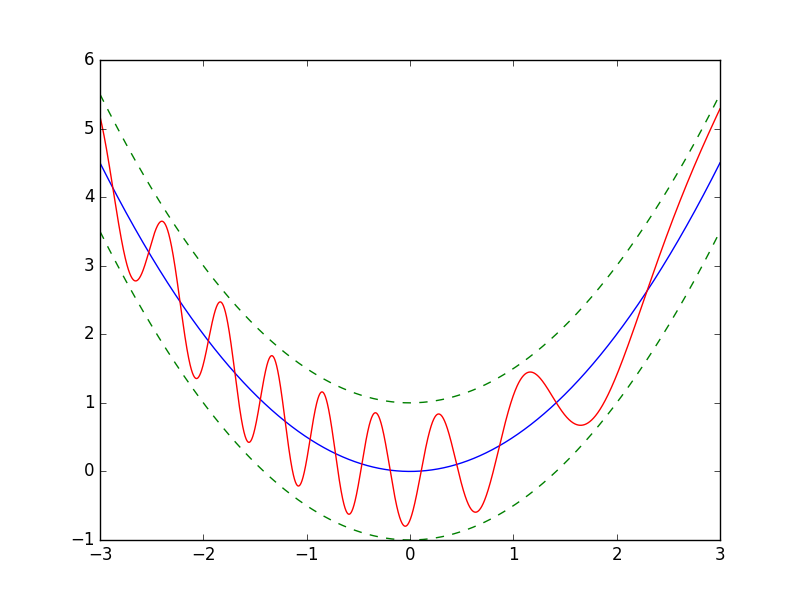
\includegraphics[scale=0.3]{2.png}
	}
	\subfigure[]{
		\label{fig:2}
		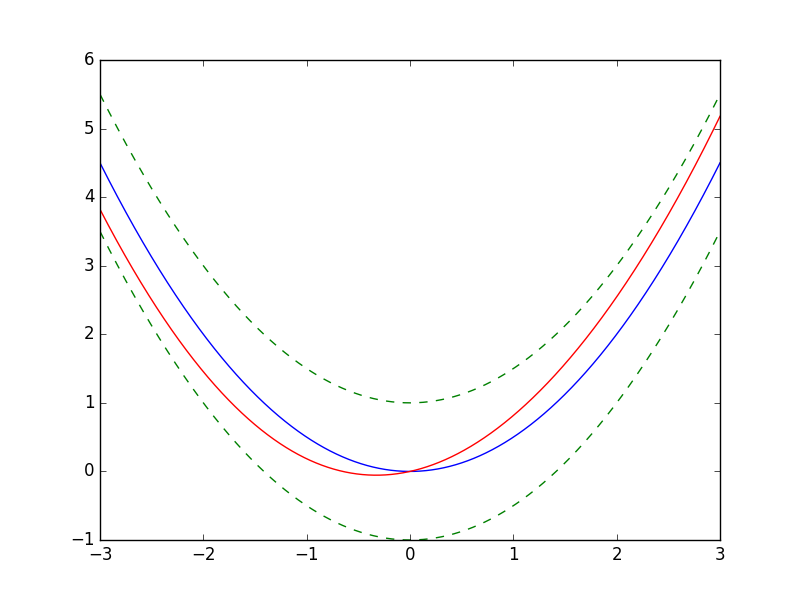
\includegraphics[scale=0.3]{3.png}
	}
	\caption{Two different empirical risk landscapes. The blue line and the red line denote the expected and training losses. The dashed green lines denote the expected loss $\pm$ $\epsilon$.}
\end{figure}

\subsection{Uniform Convergence Implies Generalization}
	Before proving uniform convergence for specific hypothesis classes, we first demonstrate how it implies generalization, i.e., an upper bound on $L(\hat h) - L(h^*)$. We can write $L(\hat h) - L(h^*)$ as
	\begin{equation}\label{eq:decomp}\begin{split}
		L(\hat h) - L(h^*)
	=	&\left[L(\hat h) - \hat L(\hat h)\right] + \left[\hat L(\hat h) - \hat L(h^*)\right] + \left[\hat L(h^*) - L(h^*)\right]\\
	\le	&\left|L(\hat h) - \hat L(\hat h)\right| + 0 + \left|\hat L(h^*) - L(h^*)\right|
	\le	2\sup_{h \in \H}\left|\hat L(h) - L(h)\right|.
	\end{split}\end{equation}
	Here the second step applies the definition of $\hat h$, and the third step follows directly from the definition of supremum.

	By Equation~\eqref{eq:decomp}, we have the following implication
	\begin{equation}\label{eq:imp}
				\forall h \in \H, \left|\hat L(h) - L(h)\right| \le \epsilon
	\implies 	\sup_{h \in \H}\left|\hat L(h) - L(h)\right| \le \epsilon
	\implies 	L(\hat h) - L(h^*) \le 2\epsilon.
	\end{equation}
	Therefore, if we could prove uniform convergence~\eqref{equation:uc} for hypothesis class $\H$, we have
	\[
		\Pr\left[L(\hat h) - L(h^*) \le 2\epsilon\right]
	\ge	\Pr\left[\forall h \in \H, \left|\hat L(h) - L(h)\right| \le \epsilon\right]
	\ge	1 - \delta,
	\]
	a generalization bound that we desire.

\subsection{Finite Hypothesis Classes}
	Now we prove that uniform convergence indeed holds for finite hypothesis classes. Recall that $n$ is the number of examples drawn i.i.d. from the data distribution, and the probability is always taken over the randomness in training examples.

	\begin{theorem}\label{thm:finite-H}
		If $\H$ is finite and $\ell((x, y), h) \in [0, 1]$, we have the following statements:
		\begin{enumerate}[(1)]
			\item \label{stmt:1} For any fixed $h \in \H$ and $\epsilon > 0$,
				\[\pr{}{\left|\hat L(h) - L(h)\right| \le \epsilon} \ge 1 - 2e^{-2n\epsilon^2}.\]
			\item \label{stmt:2} For any $\epsilon > 0$,
				\[\pr{}{\forall h \in \H,\left|\hat L(h) - L(h)\right| \le \epsilon} \ge 1 - 2\left|\H\right|e^{-2n\epsilon^2}.\]
			\item \label{stmt:3} With probability at least $1 - \delta$, for any $h \in \H$,
				\[\left|\hat L(h) - L(h)\right| \le \sqrt{\frac{\ln|\H| + \ln\frac{2}{\delta}}{2n}}.\]
			\item \label{stmt:4} With probability at least $1 - \delta$,
				\[L(\hat h) - L(h^*) \lesssim \sqrt{\frac{\ln|\H| + \ln\frac{1}{\delta}}{n}}.\]
		\end{enumerate}
	\end{theorem}

	The proof of the theorem relies on the following concentration inequality, which is a quantitative version of the central limit theorem.

	\begin{lemma}[Hoeffding's inequality]\label{lem:Hoeffding}
		Let $X_1, X_2, \ldots, X_n$ be independent random variables such that $a_i \le X_i \le b_i$ almost surely for each $i \in [n]$. Then, for any $\epsilon > 0$,
			\[\pr{}{\left|\frac{1}{n}\sum_{i=1}^{n}X_i - \Ex{}{\frac{1}{n}\sum_{i=1}^{n}X_i}\right| \le \epsilon} \ge 1 - \exp\left(-\frac{2n^2\epsilon^2}{\sum_{i=1}^{n}(b_i-a_i)^2}\right).\]
	\end{lemma}

	Now we are ready to prove Theorem~\ref{thm:finite-H}. We first prove Statement~\eqref{stmt:1} using Hoeffding's inequality, then we show that each statement directly implies the next.

	\begin{proof}[Proof of Theorem~\ref{thm:finite-H}]
		Statement~\eqref{stmt:1} follows from Hoeffding's inequality by taking $X_i = \ell((x^{(i)}, y^{(i)}), h)$, $a_i = 0$ and $b_i = 1$ for each $i \in [n]$ in Lemma~\ref{lem:Hoeffding}.
		Then, Statement~\eqref{stmt:2} follows from a union bound:
		\begin{align*}
			\pr{}{\exists h \in \H, \left|\hat L(h) - L(h)\right| > \epsilon}
		\le	&\sum_{h \in \H}\pr{}{\left|\hat L(h) - L(h)\right| > \epsilon}\tag{union bound}\\
		\le	&\sum_{h \in \H}2e^{-2n\epsilon^2}
		=	2\left|\H\right|e^{-2n\epsilon^2}.\tag{Statement~\eqref{stmt:1}}\\
		\end{align*}
		Statement~\eqref{stmt:3} follows from plugging
			$\epsilon = \sqrt{\frac{\ln\left|\H\right|+\ln\frac{2}{\delta}}{2n}}$
		into Statement~\eqref{stmt:2}.
		Finally, Statement~\eqref{stmt:3} and the implication in Equation~\eqref{eq:imp} imply Statement~\eqref{stmt:4}.
	\end{proof}

\section{Digression: The PAC Learning Framework}
	Probably approximately correct (PAC) learning is a theoretical framework of machine learning proposed by Valiant~\cite{valiant1984theory}. One of the key definitions in PAC learning is the notion of PAC learning algorithms.
	\begin{definition}[PAC learning algorithm]\label{def:PAC}
		Algorithm $\A$ is a PAC learning algorithm for hypothesis class $\H$, if for any distribution $P$ over $\X \times \Y$, $\epsilon > 0$ and $\delta \in (0, 1)$,
			\[\hat h = \A\left(\left(x^{(1)}, y^{(1)}\right), \left(x^{(2)}, y^{(2)}\right), \ldots, \left(x^{(n)}, y^{(n)}\right)\right)\]
		satisfies
		\begin{equation*}
			\pr{}{L(\hat h) - L(h^*) > \epsilon} \le \delta,
		\end{equation*}
		and $\A$ runs in polynomial time with respect to $\size(\X)$, $\frac{1}{\epsilon}$ and $\frac{1}{\delta}$.
	\end{definition}
	\begin{remark}
		Informally, $\size(\X)$ is the number of bits to describe an element of $\X$. For example, $\size(\X) = \log_2|\X|$ if $\X$ is finite. In the general case where $\X$ is parametrized by real numbers, this definition requires $\X$ to be discretized first.
	\end{remark}
	\begin{remark}
		Definition~\ref{def:PAC} implicitly requires the number of training examples, $n$, to be polynomial in $\size(\X)$, $\frac{1}{\epsilon}$ and $\frac{1}{\delta}$. Otherwise, $\A$ does not have enough time to read its entire input.
	\end{remark}

	One limitation of Valiant's framework is that it requires the algorithm to work on \emph{every} data distribution $P$, which turns out to be overly ambitious and thus unrealistic. In contrast, recent research on learning theory usually requires certain assumptions on the data distribution, e.g., the distribution is Gaussian or realizable (i.e., the hypothesis class contains the function to be learned).

	Thus, it is worth thinking about the role of assumptions on learning theory research. Suppose we could prove the following three theorems:
	\begin{itemize}
		\item \textbf{Theorem A.} Statement $P$ implies Statement $Q$.
		\item \textbf{Theorem B.} Under certain assumptions, $P$ implies $Q$.
		\item \textbf{Theorem C.} Under certain assumptions, $P$ implies a statement stronger than $Q$.
	\end{itemize}
	Theorem~B is definitely the weakest among these three, yet Theorems A~and~C are incomparable. It is often a matter of taste whether one prefers $A$ or $C$. In deep learning theory, however, Statement $Q$ is often vacuous for most practical uses. In this case, we had better prove a result similar to Theorem~C, and then find out how the assumptions can be weakened and eventually removed.

\bibliographystyle{alpha}
\bibliography{10_01_final}

%%%%%%%%%%%%%%%%%%%%%%%%%%%%%%%%%%%%%%%%%%%%%%%%%%%%%%%%%%%%%%%%

\end{document}
